\chapter{Reinforcement Learning}

Reinforcement learning (RL) is all about the interaction between agent and environment. The learning comes in the form of trial-and-error, in which the agent observe the state of the environment, takes actions according to that observations, influencing new possible states configurations, and perceive rewards given its previous decision. Everything is commanded toward achieve a goal such as escaping from a maze, \href{https://arxiv.org/abs/1312.5602}{win some Atari Game} \citep{mnih2013playing}, or \href{https://deepmind.google/technologies/alphago/}{defeating the world champion of Go} \citep{silver2016mastering}. The reward is how we encoded our progression to the goal.

\section{The Framework for Learning to Act}

\begin{figure}[ht]
    \centering
    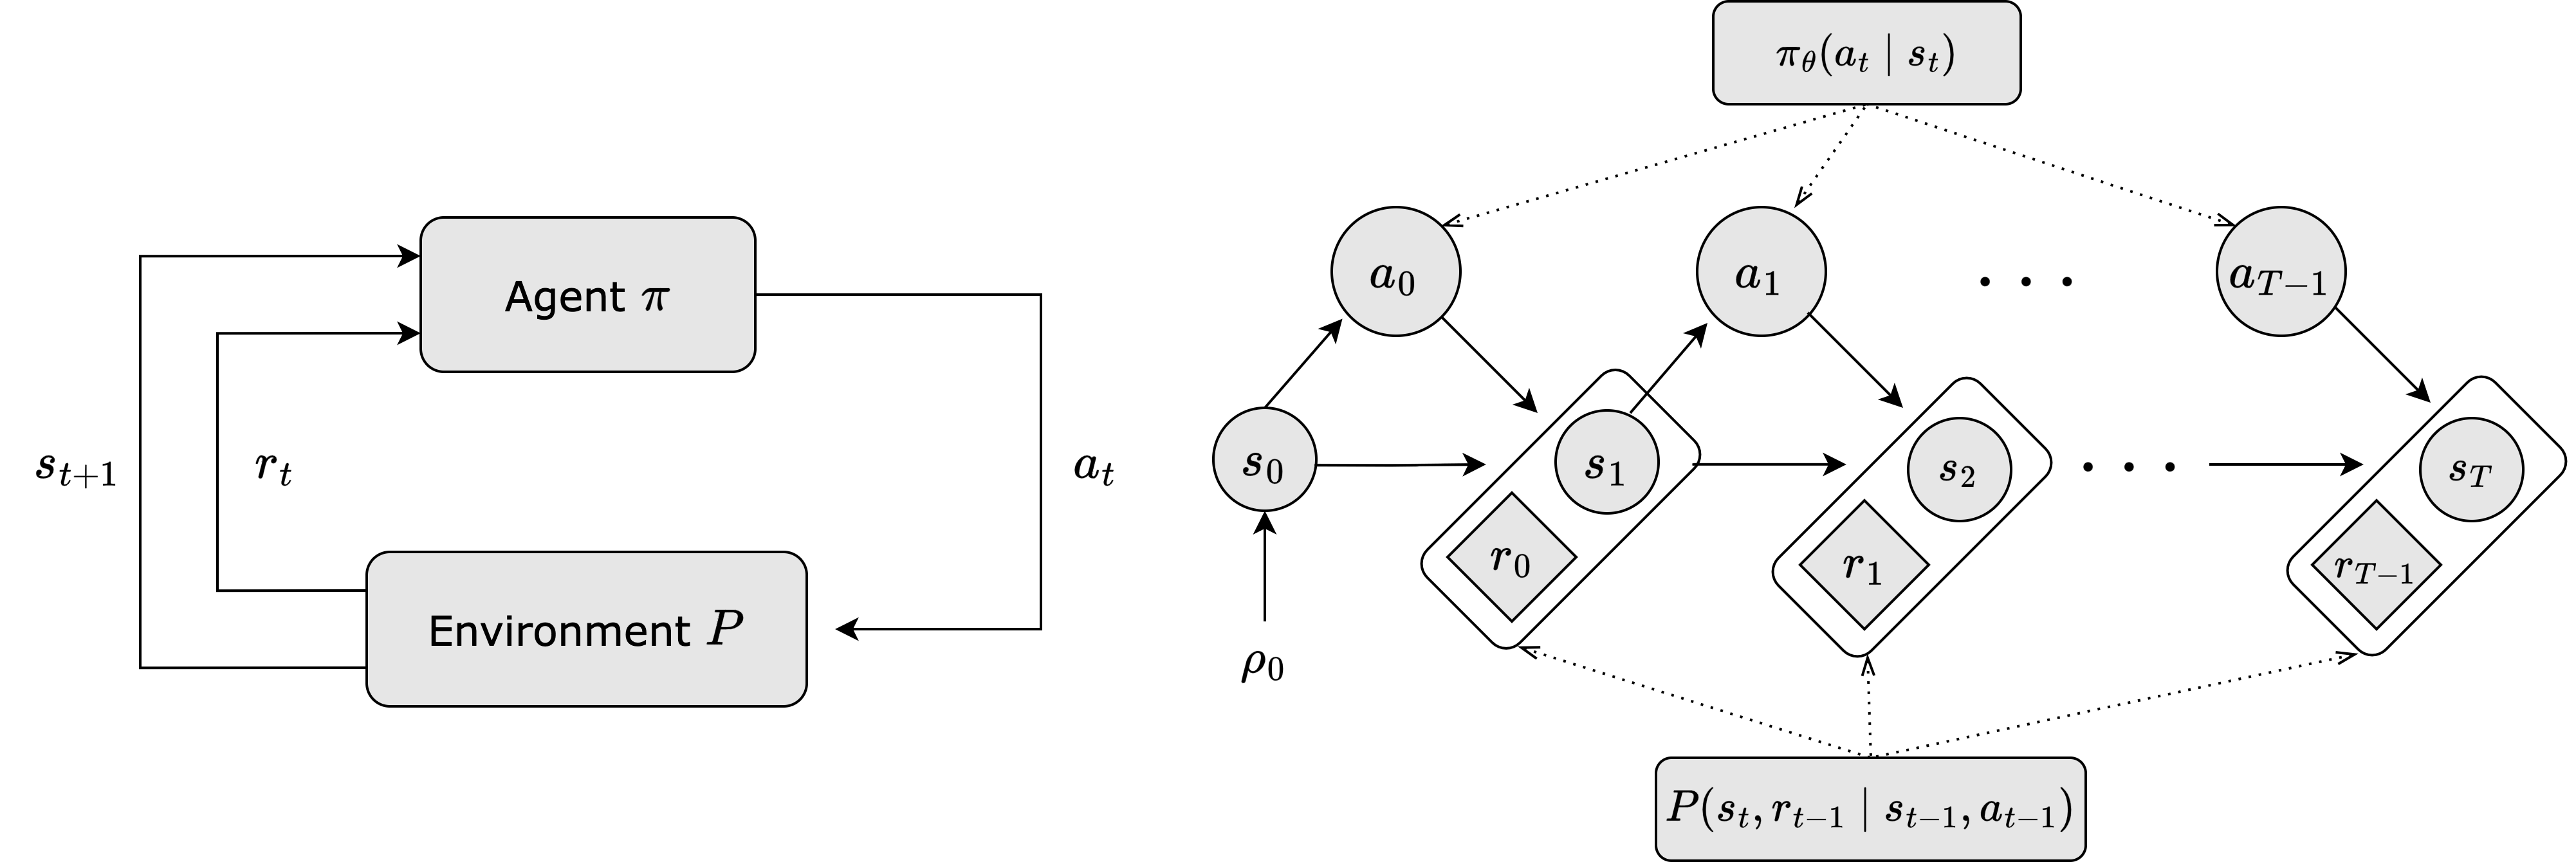
\includegraphics[scale=0.65]{ch3-rl/MDP-diagram.png}
    \captionsetup{width=\textwidth} % set the width of the caption
    \caption{\textbf{Left:} a Markov Decision Process (MDP) loop representation. \textbf{Right:} An unrolled MDP representing an episodic case with a finite horizon $T$, and a paramterized policy $\pi$ by $\theta$.}
    \label{fig:mdp-diagram}
  \end{figure}

Introducir toda la notación...

Si el agente tiene acceso o no al modelo del ambiente: model-free RL y model-based RL. Disponer de un model del mundo permite al agente planificar. 
En cambio, model-free RL son mas fáciles de implementar, pero están
sujes a las dificultades de solo poder muestrear para aprender a 
actuar.

The Markov Decision Processes (MDP) is at the core of reinforcement Learning as the mathematical object in which RL built on top of it. An MDP is a sequence of state-actions that model the agent interaction with the environment under the Markovian property, which states that the future and the past are
conditionally indepeendent, given the present (memoryless). Every information we
need to determine the future states are in the present.

Here we will introduce the notation to describe an MDP:

\section{Proximal Policy}

Represent the agent with a function approximator, and we will use a deep neural network for it. That's the reason why are people that call this subfield of reinforcement learning Deep Reinforcement Learning...

The policy is a distributions over actions spawned conditional the states.

\textbf{TODO:} Introduce what we want to maximize, the expected return of the trajectory, and the gradient estimation via score function.

\subsection{Learning the Policy}

The main difference between Supervised Learning and Reinforcement Learning is that we don't have a direct feedback of each action through a label. Even in the case that we have a label for an action, we're just not simply interested in the evaluation of individual actions, instead we are interested in the overall trajectory performance, and intertwined of states $s_t$ and actions $a_t$. So, how can we obtained feedback for backpropagated it through agent's parameters to provide corrections about its actions?

The starting point is thinking in trajectories as a unit of learning, instead of individual observations (i.e. actions). What is the dynamic that instance/spawn a trajectory? Given a policy $\pi_{\theta}$, represented as a function with parameter $\theta$, we can deployed the agent into their environment at an initial state $s_0$ and look up--just in inference mode or \textit{evaluation phase}-how does promote actions $a_t$ given the current state $s_t$, repeatedly, until we have an episode $t=T$. In which we can know if the goal was accomplished or not, i.e. we won the ATARI pong game? or does the drone achieve stability in the flight, given the initial settings? or \textit{my samples from the diffusion model are enough aesthetic as I want?} The reward we will provide signal to us about if we met the ultimate goal, and we can just think of the signal as a "proxy of a label", but for the overall trajectory. That it is the job of the \textbf{return function} (check terminology), collapse the rewards obtained during trajectory into a single scalar that provides a measure of assessment whether the agent achieve their goal or not. Therefore, we end up with a "proxy label" for our unit learning that is the trajectory. The remaining job is to establish the feedback mechanism to the \textit{learning phase}.

Mathematically we want to perform a stochastic optimisation to learn the agent's parameters, i.e. obtained gradient information from the trajectory's under the performance given a scalar-value function that provide assessment (aka reward). Stochastic because both, the agent and environment has elements of randomness, and for this reason we can just compute estimates from the reward trajectory and estimates of the gradient. So, we will need to take a short detour in the realm of Monte Carlo Gradient Estimation \citep{mohamed2020monte}. \textbf{CHECK}: Notice that from the machine learning point of view, we were performing a double optimization, once associated by the stochasticity of the samples to estimate the gradient, and the other for the gradient descent algorithms used by update the parameters.

\section{Gradient Estimation via Score Function}

The gradient estimation can be obtained using the score function gradient estimator. Let's introduce the following general probability objective $\mathcal{F}$, defining in the \href{https://en.wikipedia.org/wiki/Ambient_space_(mathematics)}{ambient space} $\mathcal{X}\in\mathbb{R}^n$ and $\theta\in\mathbb{R}^n$,

\begin{equation}\label{eqn:probability-objective}
\mathcal{F}(\theta) = \int_{\mathcal{X}} p(\mathrm{x; \theta})f(\mathrm{x})~d\mathrm{x} = \mathbb{E}_{p(\mathrm{x};\theta)}\big[f(\mathrm{x})\big]
\end{equation}

Here, $f$ is scalar-valued function, similar to how the reward is represented
in the reinforcement learning setting. The \textit{score function} is the derivative of
the log probability distribution $\nabla_{\theta}\log p(\mathrm{x};\theta)$ w.r.t. its parameters $\theta$. We
can summon it via the following identity that establish a connection between
the score function and the probability distribution $p(\mathrm{x};\theta)$.

\begin{equation}\label{eqn:log-derivative-trick-expression}
    \begin{split}
        \nabla_\theta\log p(\mathrm{x};\theta) &= \frac{\nabla_{\theta}p(\mathrm{x}; \theta)}{p(\mathrm{x};\theta)} \\
        p(\mathrm{x};\theta) \nabla_{\theta}\log p(\mathrm{x};\theta) &= \nabla_{\theta}p(\mathrm{x};\theta)
    \end{split}
\end{equation}

Therefore, taking the gradient from the objective $\mathcal{F}(\theta)$ w.r.t. the parameter $\theta$ we have

\begin{equation}
    \begin{split}
        \eta = \nabla_{\theta} \mathbb{E}_{p(\mathrm{x};\theta)}[f(\mathrm{x})] &= \nabla_{\theta}\int_{\mathcal{X}} p(\mathrm{x};\theta) f(\mathrm{x}) d\mathrm{x} \\
        &= \int_\mathcal{X} \nabla_{\theta}~p(\mathrm{x}; \theta)f(\mathrm{x})d\mathrm{x} \\
        &= \int_{\mathcal{X}}p(\mathrm{x};\theta)\nabla_{\theta}\log p(\mathrm{x}; \theta) f(\mathrm{x})d\mathrm{x} \\
        &=\mathbb{E}_{p(\mathrm{x};\theta)}\big[f(\mathrm{x})\nabla_{\theta}\log p(\mathrm{x};\theta) \big] 
    \end{split}
\end{equation}

The use of the log-derivative rule in \ref{eqn:log-derivative-trick-expression} to make appear the score function is also known as the
\href{https://blog.shakirm.com/2015/11/machine-learning-trick-of-the-day-5-log-derivative-trick/}{\textit{log-derivative trick}}.
Now, we can compute an estimate of the gradient, $\bar{\eta}$, using Monte Carlo samples from the distribution $p(\mathrm{x};\theta)$, as follows, 

\begin{equation}\label{eqn:score-function-gradient-estimator}
    \bar{\eta}_{N} = \frac{1}{N}\sum_{i=1}^{N}f\big(\hat{\mathrm{x}}^{(i)}\big) \nabla_{\theta}\log p\big(\hat{\mathrm{x}}^{(i)};\theta\big)
\end{equation}

We draw $N$ samples $\hat{\mathrm{x}}\sim p(\mathrm{x};\theta)$, and compute the gradient of the log-probability of each sample, and multiply by the scalar-valued function $f$ evaluated at the sample. The average of these terms is an unbiased estimate of the gradient of the objective $\eta$. \\

There are two points worth to mention about Eq.~\ref{eqn:score-function-gradient-estimator}.

\begin{enumerate}
    \item The function $f$ can be any arbitrary function we can evaluate on $\mathrm{x}$, even if it's not differentiable w.r.t $\theta$, it will work for compute the gradient estimation $\bar{\eta}$. \textbf{TODO:} revisar la precisión de esto...
    \item Expectation of the score is $0$, that is,
    \begin{equation}\label{eqn:score-function-expectation-zero}
    \begin{split}
        \mathbb{E}_{p(\mathrm{x};\theta)}\big[\nabla_{\theta}\log p(\mathrm{x};\theta)\big] 
        &= \int_{\mathcal{X}}p(\mathrm{x};\theta)\nabla_{\theta}\log p(\mathrm{x}; \theta) d\mathrm{x} \\
        &= \int_{\mathcal{X}} p(\mathrm{x};\theta)\frac{\nabla_{\theta} p(\mathrm{x}; \theta)}{p(\mathrm{x};\theta)}d\mathrm{x} \\
        &= \int_{\mathcal{X}}\nabla_{\theta}p(\mathrm{x};\theta)d\mathrm{x} \\
        &= \nabla_{\theta}\int_{\mathcal{X}} p(\mathrm{x}; \theta)d\mathrm{x} = \nabla_{\theta} 1 =0
    \end{split}
    \end{equation}
\end{enumerate}

The last point is particularly useful because we can replace $f$ by a shifted
version given a constant $\beta$, and obtain the following unbiased estimate of
the gradient estimator, which can be beneficial in the optimization task.

\begin{equation}\label{eqn:score-function-gradient-estimator-baseline}
\bar{\eta}_{N} = \mathbb{E}_{p(\mathrm{x}_{\theta})}\big[(f(\mathrm{x}) - \beta) \nabla_{\theta} \log p(\mathrm{x}; \theta)\big]
\end{equation}

Using a \textbf{\textit{baseline function}} to determine $\beta$ that doesn't
depend on the parameter $\theta$ can reduce the variance of the estimator. The
baseline function can be any function that doesn't depend on $\theta$ to
safisfy the property in Eq.~\ref{eqn:score-function-expectation-zero}, and it is used to reduce the variance of the estimator. The variance of the estimator is reduced when the baseline function is chosen to be close to the scalar-valued function $f$.

\section{Vanilla Policy Gradient, aka REINFORCE}

REINFORCE \citep{williams1992simple} is the translation of the above derivation
of the gradient estimation via score function in reinforcement learning 
parlance.

We are in the setting of Policy Gradient algorithms, in which the objective is
to maximize the expected return of the trajectory $\tau$ under the policy 
$\pi$ parameterized by $\theta$ (e.g. a neural network). At each state
$s_t$ the agent takes an action $a_t$ according to the policy $\pi$,
which spawn a probability distribution over actions $\pi(a_{t}~|~s_{t};~\theta)$. For here, we will use the notation $\pi_{\theta}(\cdot)$ instead of 
$\pi(\cdot;~\theta)$.

As we mentioned in previous section, the trajectory $\tau$ represent the
pairs of action-state arise from the agent interaction with their environment. 
From the initial state $s_{0}$ to the terminal state $s_{T}$, the trajectory
$\tau$ is a sequence of states and actions, $\tau = (s_{0}, a_{0}, \dots, s_{T-1}, a_{T-1}, s_{T})$, which tell us the story of how the agent
act during the episodic task. Let's introduce $p_{\theta}(\tau)$ as the
probability to obtain the trajectory $\{\tau^{(i)}\}$ under the policy $\pi_{\theta}$. \\

So we have a distribution of trajectories. Remember that the unit of learning
is the trajectory $\tau$, and the goal is to maximize the expected return of the
trajectory. The return $R(\tau)$ could be the cumulative rewards obtained during the \textit{episode}, or the discounted rewards. The expected return is given by the following expression,

\begin{equation}\label{eqn:rl-objective}
    \mathbb{E}_{p_{\theta}(\tau)}[R(\tau)] 
\end{equation}

This is the objective we want to maximize, and is a 
particular case of Eq.~\ref{eqn:probability-objective} with the
scalar-valued function $f(\tau) = R(\tau)$, the return of the trajectory. 
Lets use the tricks of the previous section to compute the
gradient of the objective in Eq.~\ref{eqn:rl-objective} w.r.t. the policy
parameter $\theta$. The gradient estimation is given by,

\begin{equation}\label{eqn:rl-gradient-estimator-vanilla}
    \nabla_{\theta} \mathbb{E}_{p_{\theta}(\tau)}[R(\tau)] = \mathbb{E}_{p_{\theta}(\tau)}\big[R(\tau)\nabla_{\theta}\log p_{\theta}(\tau)\big]
\end{equation}    

What exactly is $p_{\theta}(\tau)$? Given that the trajectory is a sequence of
states and actions, and under the Markovian assumption imposed by the MDP, the
probability of the trajectory is 

\begin{equation}\label{eqn:trajectory-probability-expanded}
    \begin{split}
        p_{\theta}(\tau) &= p_\theta(s_{0}, a_{0}, s_{1}, a_{1}, \dots, s_{T-1}, a_{T-1}, s_{T}) \\
        &= \rho(s_0)~\prod_{t=0}^{T-1} \pi_{\theta}(a_{t}~|~s_{t})~P(s_{t+1}, r_{t}~|a_{t}, s_{t})
    \end{split}
\end{equation}

The magic happens when we take the log of the probability of the trajectory, and
the gradient of this log-probability w.r.t. the policy parameter $\theta$,

\begin{equation}\label{eqn:trajectory-gradient-score}
    \begin{split}
        \log p_{\theta}(\tau) &= \log \rho(s_0) + \sum_{t=0}^{T-1}\log \pi_{\theta}(a_{t}~|~s_{t}) + \log P(s_{t+1}, r_{t}~|a_{t}, s_{t}) \\
        \nabla_{\theta}\log p_{\theta}(\tau) &= \sum_{t=0}^{T-1}\nabla_{\theta}\log \pi_{\theta}(a_{t}~|~s_{t})
    \end{split}
\end{equation}

The distribution of initial states $\rho(s_{0})$ and the transition
probabilities $P(s_{t+1}, r_{t}~|~a_{t}, s_{t})$ are eliminate for not depend
on $\theta$, simplifying the required computations needed to estimate the
gradients. Plugging the final expression of Eq.~
\ref{eqn:trajectory-gradient-score} in the gradient estimation of the objective
in Eq.~\ref{eqn:rl-gradient-estimator-vanilla}, we have the REINFORCE gradient
estimator,
\begin{equation}\label{eqn:reinforce-gradient-estimator}
    \nabla_{\theta}\mathbb{E}_{p_{\theta}(\tau)}[R(\tau)] = \mathbb{E}_{p_{\theta}(\tau)}\bigg[R(\tau)\bigg(\sum_{t=0}^{T-1} \nabla_{\theta}\log \pi_{\theta} (a_t~|~s_t) \bigg)\bigg] 
\end{equation}

%\begin{equation}\label{eqn:reinforce-gradient-estimator2}
%    \nabla_{\theta}\mathbb{E}_{p_{\theta}(\tau)}[R(\tau)] = \mathbb{E}_{p_{\theta}(\tau)}\bigg[\bigg(\sum_{t=0}^{T}R(s_{t}, a_{t})\bigg) \bigg(\sum_{t=0}^{T-1} \nabla_{\theta}\log \pi_{\theta} (a_t~|~s_t) \bigg)\bigg] 
%\end{equation}

The idea is to collect a trajectory and update the policy parameters $\theta$ to increase the likelihood of high-reward trajectories while decreasing the likelihood of low-reward ones. This trial-and-error learning approach, involves adjusting the policy parameters based on the trajectory's goodness, making good trajectories more probable and less desirable ones less so.
\begin{figure}[ht]
    \centering
    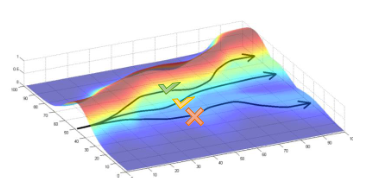
\includegraphics[scale=0.85]{ch3-rl/simulated-trajectories-levine-slides.png}
    \captionsetup{width=\textwidth} % set the width of the caption
    \caption{\textbf{Illustration of three simulated trajectories}, denoted as $\{\tau^{(i)}\}$ where $i=(1,2,3)$, traversing the parametric space $\theta\in\mathbb{R}^2$ under the policy $\pi_{\theta}$. Each trajectory is marked with a color symbol (cross, check) that represents its \textit{goodness} based on the reward function $R(\tau^{(i)})$. \textbf{Source:} \href{https://rail.eecs.berkeley.edu/deeprlcourse/}{Policy Gradients Lecture, Deep Reinforcement Learning Course} by Sergey Levine.}
    \label{fig:anatomy-rl-trajectories}
  \end{figure}

% algoritmo naive REINFORCE
\begin{algorithm}
    \caption{Vanilla Policy Gradient, aka REINFORCE}
    \begin{algorithmic}
    \STATE Initialize policy parameter $\theta$, set learning rate $\alpha$
    \STATE Generate $\tau=(s_0, a_0, ..., s_{T-1}, a_{T-1}, s_{T})$ by sampling from current $\pi_{\theta}$
    \FOR{$t=0, 1, \dots, T-1$}
        \STATE Estimate the return $R(\tau)$
        \STATE Update the policiy parameters $\theta \leftarrow \theta + \alpha~r_{t}\nabla_{\theta}\log\pi_{\theta}(a_{t}|s_{t})$
    \ENDFOR
    \end{algorithmic}
\end{algorithm}
A naive estimate of $R(\tau)$ is used the total trajectory reward, this means
that every action is weighted by the total reward, and even if the gradient
estimator is unbiased, we need to care about the variance of the estimator.
In order to reduce the variance of the estimator, we can impose causality
by using the rewards-to-go, i.e. the sum of rewards from the current time-step
to the end of the trajectory. This is a simple trick that can reduce the variance. \textbf{TODO:} ¿Porqué \textit{reward-to-go} reduce la varianza? ¿Cómo se puede
demoostrar?
\begin{equation}\label{eqn:reinforce-gradient-reward-to-go}
    \nabla_{\theta}\mathbb{E}_{p_{\theta}(\tau)}[R(\tau)] = \mathbb{E}_{p_{\theta}(\tau)}\bigg[\bigg(\sum_{t=0}^{T-1} \nabla_{\theta}\log \pi_{\theta} (a_t~|~s_t)\bigg) \bigg(\sum_{t'=t}^{T-1}R(s_{t}, a_{t}, s_{t+1})\bigg)\bigg] 
\end{equation}
Notice that 
Lets come back to the \textit{baseline}, we want to use a baseline function
based on the current $s_{t}$, because it is reduce the variance of our gradient
estimate without unbiased the estimator, i.e. at no cost.

First, it's the expectation of the score still unbiased in this setting?

\begin{equation}\label{eqn:reinforce-gradient-estimator-baseline}
    \begin{split}
        \nabla_{\theta}\mathbb{E}_{\tau} &= \mathbb{E}_{p_{\theta}(\tau)} \bigg[\sum_{t=0}^{T-1}\nabla_{\theta}\log\pi_{\theta}(a_{t}|s_{t}) \bigg( \sum_{t=t'}^{T-1} r_{t'}-b(s_{t}) \bigg) \bigg]
    \end{split}
\end{equation}

Well the proof follows the same argument that shows in Eq.~\ref{eqn:score-function-expectation-zero}, but with the difference that 
$p_{\theta}(\tau)$ is a sequence of random variables. Therefore,
the adaptation involves expanding the trajectory into state-action pairs and break this sequence into two pieces around $t$. We will show in one of the
terms  of the score function multiplied by the baseline that it has a null
effect on the expectation, as well as any other of these terms due to linearity of expectation.

\begin{equation}\label{eqn:reinforce-baseline-unbiased}
   \begin{split}
        \mathbb{E}_{p_{\theta}(\tau)}\big[\nabla_{\theta}\log\pi_{\theta}(a_t|s_t) b(s_t) \big] &= \mathbb{E}_{s_{0:t}, a_{0:t-1}}\big[\mathbb{E}_{s_{t+1:T}, a_{t:T-1}}[ \nabla_{\theta}\log \pi_{\theta}(a_{t}|s_{t})b(s_{t})]\big] \\
        &= \mathbb{E}_{s_{0:t}, a_{0:t-1}}\big[b(s_{t})\mathbb{E}_{s_{t+1:T}, a_{t:T-1}}[ \nabla_{\theta}\log \pi_{\theta}(a_{t}|s_{t})]\big] \\
        &= \mathbb{E}_{s_{0:t}, a_{0:t-1}}\big[b(s_{t})\mathbb{E}_{a_{t}}[ \nabla_{\theta}\log \pi_{\theta}(a_{t}|s_{t})]\big] \\
        &= \mathbb{E}_{s_{0:t}, a_{0:t-1}}\big[b(s_{t})\nabla_{\theta}\mathbb{E}_{a_{t}}[\log \pi_{\theta}(a_{t}|s_{t})]\big] \\
        &= \mathbb{E}_{s_{0:t}, a_{0:t-1}}\big[b(s_{t})\nabla_{\theta}1\big] = 0
   \end{split}
\end{equation}

We know that introducing a baseline keeps the estimator unbiased, but why
the baseline can reduce the variance of the estimator? In \cite{seita2017going}
there is an explanation of how to rearrange the variance of the score function and queda formulado una esperanza factorizada donde esta el retorno menos el baseline. De poder optimizarse, se puede formular como least square error, y
la función de baseline ideal sería estimar el retorno esperado. Así sabemos
si el retorno esta sobre o bajo el retorno esperado, y reduciendo la varianza 
del estimador al mismo tiempo...preguntar sobre manipulación de la esperanza...
y agregar formulación!


\section{Deep Reinforcement Learning}

The REINFORCE algorithm is a simple and powerful algorithm to learn the policy,
even more when we equipped the agent with a neural network as a function 
approximation of the policy. 

\textbf{TODO:} Implement the REINFORCE algorithm in a simple environment, such as ATARI PONG game. Focus to highlight the following:

\begin{enumerate}
    \item The policy is a neural network that takes the state as input and output a distribution over actions, i.e. softmax layer.  
    \item Using automatic differentiation as engine to backpropagate the gradient estimation. We need a loss function to compute the gradient, how
    can we convert the Eq.~\ref{eqn:reinforce-gradient-estimator} into a loss?
    \item Take advantage of neural network to learn useful representations from raw data such as images (e.g. convolutions).
\end{enumerate}

\begin{equation}\label{eqn:neural-softmax-policies}
    \pi_{\theta}(a~|~s) = \frac{\exp(f_{\theta}(s, a))}{\sum_{a'\in\mathcal{A}}\exp(f_{\theta}(s, a'))}
\end{equation}

In the previous section we see how to get an expression to estimate the gradients. However, in practice, where we use complex function
$f_{\theta}$ to approximate our policy $\pi$, we want to express a cost
function $\mathcal{J}(\theta)$ in a manner that we can take advantange of 
automatic differentiation engines such as PyTorch or JAX.

\begin{equation}\label{eqn:reinforce-gradient-estimator-cost}
    \mathcal{J}(\theta) = \mathbb{E}_{p_{\theta}(\tau)}\bigg[R(\tau)\bigg(\sum_{t=0}^{T-1} \log \pi_{\theta} (a_t~|~s_t) \bigg)\bigg] 
\end{equation}

We will use a convolutional neural network design to learn features from
raw input such as RGB images or video frames. Without any prior information about the ATARI game more than the inductive bias of the neural network tailord to process images, we will learn a policy that maximize the reward, i.e. win
the game.

The preprocessing regarding the raw Atari images is from $210\times 160$ pixel 
images

Regarding the preprocessing of the raw Atari images, we follow the instructions
from the work playing atari games \cite{mnih2013playing}. It consist in
apply to the $210\times 160$ images a 2 factor down-samplig to $110\times 84$
and from RGB to grayscale. The resulted images were cropped into a $84\times84$
region of the pixels that represent the ``playing area''.

\section{Limitations of REINFORCE}

Higher variance, not allow to update the parameter in batches...

\subsection{Baseline}

As we see...one easy way to reduce the variance is add the following
baseline $\beta=\frac{1}{N}\sum_{i=1}^{N} r(\tau)$.

\section{Proximal Policy Optimization (PPO)}

Uno de los problemas de algoritmos tipo REINFORCE es la alta varianza del
estimador del gradiente. Un método que estudiamos para reducir la varianza
es el uso de baselines. Sin embargo, cabe mencionar otra línea de problemas
con este tipo de algoritmos \textit{model-free}, el de sampling efficiency. Una
vez que actualizamos los parámetros $\theta$ con el dataset de trayectorias,
debemos volver a muestrear, y no es posible reutilizar estas muestras porque
ya noo pertenecen a la distribución. Es decir, la distribución del dataset
$\mathcal{D}$ de trayectorias $\{\tau_i\}$ es no-estacionario, lo que dificulta
técnicas regulares usadas en supervised learning.

Estoo es porque el algoritmo es on-policy, cómo podemos ajustar el
algoritmo a off-policy? Esto significa sampleaer de otra distribución.


\subsection{Importance Sampling}


Using importance sampling we can estimate the expectation $\mu$ of a random
variable $f(x)$ under a distribution $p$ from samples of a different 
distribution $q$. 


\subsection{Bound...}

\section{Summary}

In a summary, solve a reinforcement learning problem
via proximal policy...